\documentclass{article}

\usepackage{graphicx}
\usepackage{pdflscape}
\usepackage[pass]{geometry}
\setlength{\parskip}{1em}

\begin{document}

	\title{EMISY project report:\\Thermal-paper-based optical storage medium
	reading device}
	\author{Michał Szopiński\\\\
	https://github.com/Lachcim/szopinski-emisy}
	\date{April 2, 2021}
	\maketitle
	
	\setcounter{section}{-1}
	\section{Abstract}
	
	The goal of this project was to design a device capable of reading binary
	data from a tape of 80-millimeter thermal paper on which information is
	encoded as a series of black and white squares. The device was to
	communicate with the host computer over the Universal Serial Bus, which
	would enable the data to be collected and recorded by a dedicated computer
	program.
	
	Described in this document are the engineering challenges faced during the
	construction of the machine as well as detailed descriptions of their
	solutions. The project was successfully completed using real hardware.
	
	\newpage
	\newgeometry{left=2.5cm,right=2.5cm}
	
	\hspace{0cm}
	\vfill
	\begin{figure}[h]		
		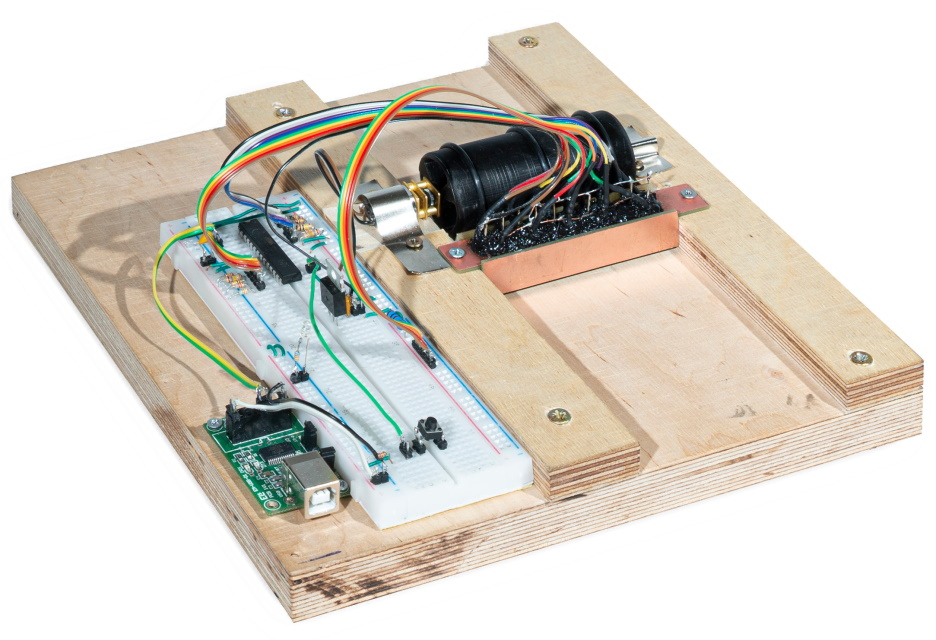
\includegraphics[width=\linewidth]{img/device}
		\caption{A photo of the device.}
	\end{figure}
	\vfill
	\hspace{0cm}
	
	\restoregeometry
	
	\newpage
	\renewcommand{\baselinestretch}{0}\normalsize
	\tableofcontents
	\renewcommand{\baselinestretch}{1}\normalsize
	
	\newpage
	\section{Introduction}
	
	Among the first storage media ever used in computing were punched cards and
	punched tape. Although simple in concept, these media are difficult to read
	quickly and accurately using analog circuitry alone. Combining the
	straightforwardness of the past with the robustness of the present, a
	simple microcontroller system may be devised to ensure that they are
	processed in a swift and reliable manner.
	
	To simplify and accelerate the production of sample media to be used with
	the device, thermal paper was chosen in place of the punched tape. Owing to
	the ubiquity and simplicity of generic point-of-sale linear thermal
	printers, any modern computer may be used to produce data tapes without the
	need for any additional drivers.
	
	Both reading and writing of the data tapes is achieved using a simple
	command line interface utility named \texttt{thermfile}, which comes
	bundled with the source code for this project. The implementation of said
	program is outside the scope of this document.
	
	\subsection{Description of the data format}
	\label{sec:format}
	
	Below is an illustration showing an example data tape with an explanation
	of its characteristic features. As the device pulls the tape through the
	read head, the symbols are scanned from top to bottom.
	
	As seen on figure~\ref{fig:horizontal}, the tape is split into 10
	machine-readable data tracks and an extra human-readable text track. The
	leftmost 8 tracks encode the 8 bits of a byte, with the least significant
	bit towards the right. The text track provides a handy reference as to what
	data is represented by each symbol.
	
	Because the machine has no control over the absolute position of the tape
	and can only approximately control its speed, a synchronization signal must
	be introduced to ensure that the symbols are read correctly. A pattern of
	alternating ones and zeros is printed on the sync track, marking the start
	and end of a symbol.
	
	Finally, the invert track is used to signify that the data bits of a symbol
	are logically inverted, i.e., ones are represented by zeros and vice-versa.
	This is due to a technical limitation of thermal printers whereby an
	excessive burn area causes a voltage drop in the printer's power rail,
	deteriorating the printout quality. The invert track ensures that at most
	50\% of horizontal space is only ever utilized.
	
	\begin{landscape}
		\begin{figure}[h]
			\minipage{0.5\textwidth}
				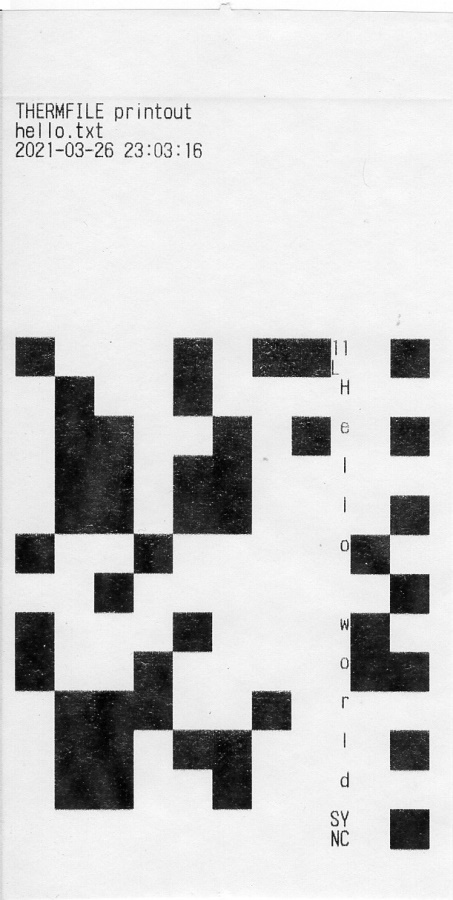
\includegraphics[width=\linewidth]{img/helloworld}
				\caption{Sample data tape}
			\endminipage\hfill
			\minipage{0.5\textwidth}
				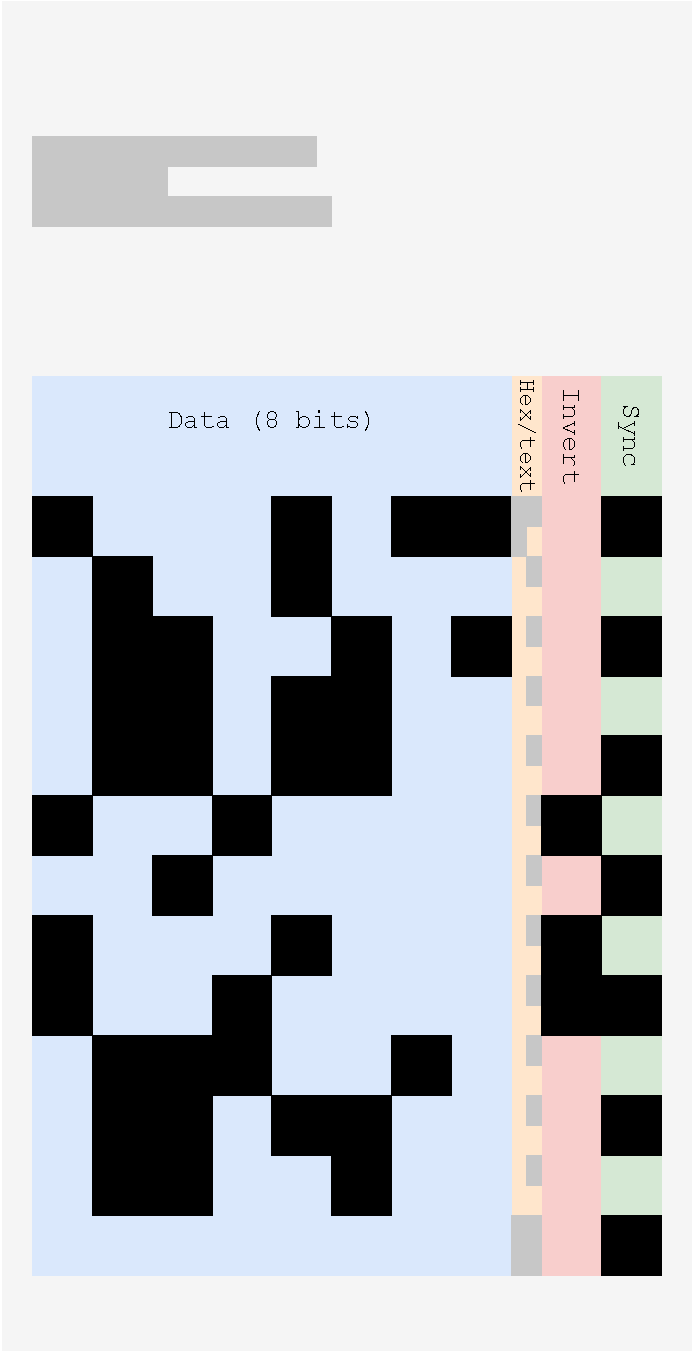
\includegraphics[width=\linewidth]{img/horizontal}
				\caption{Horizontal layout}
				\label{fig:horizontal}
			\endminipage\hfill
			\minipage{0.5\textwidth}
				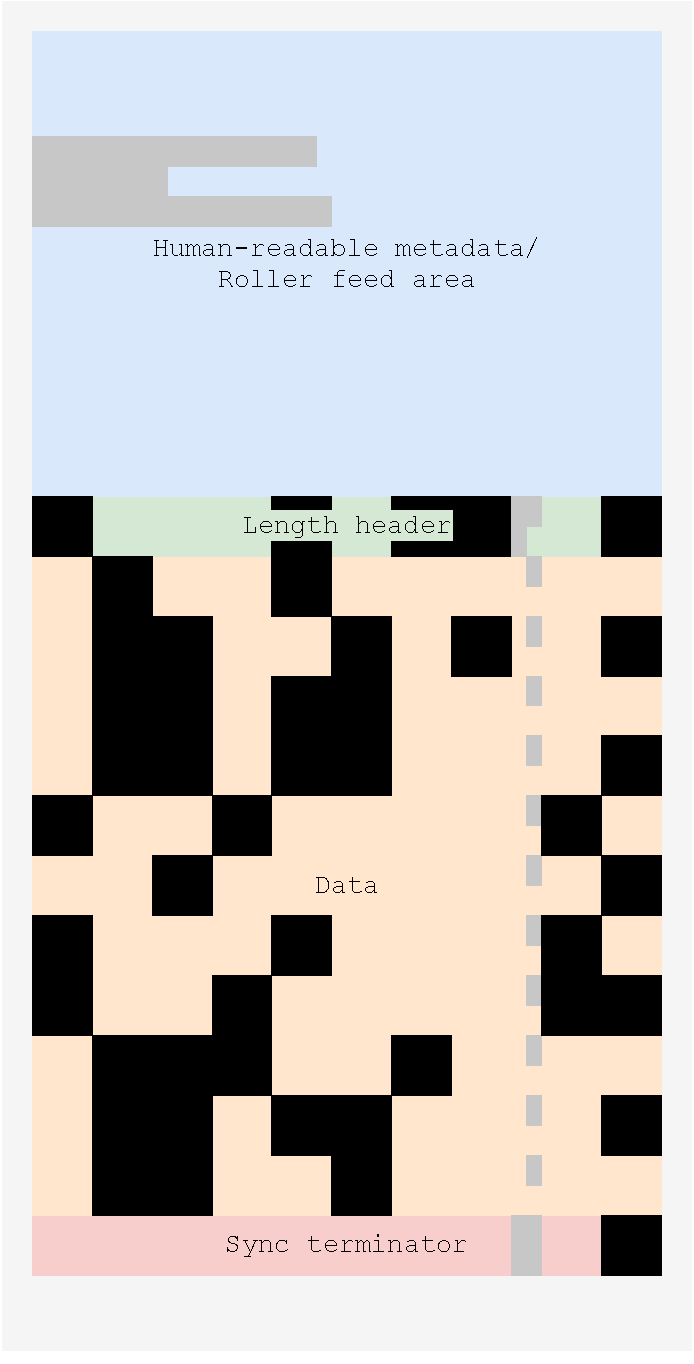
\includegraphics[width=\linewidth]{img/vertical}
				\caption{Vertical layout}
				\label{fig:vertical}
			\endminipage
		\end{figure}
	\end{landscape}
	
	Figure~\ref{fig:vertical} shows the vertical layout of symbols on the tape.
	Each printout begins with a large blank area on which human-readable
	metadata is printed for convenience. This area allows the user to push the
	tape through the read head chamber, past which it can be taken up by the
	roller. It also participates in the two-step read initialization process
	discussed in section~\ref{sec:software}.
	
	As a simple error detection measure, the device is informed about the
	length of the incoming data in advance. This information is carried by the
	length header, present at the start of the data track. Each line of the
	header carries 7 bits of the length value, in little endian order. The
	most significant bit marks the end of the length header.
	
	Past the header, binary data begins. The start and end positions of a
	symbol are determined by detecting a change in the synchronization signal.
	If there is an odd number of symbols on the tape, the final sync signal is
	white and therefore indistinguishable from the white margin of the tape.
	For this reason, a sync terminator is introduced to mark the end of
	odd-numbered final symbols.
	
	\subsection{Communication protocol}
	
	Having no hardware resources required for independent operation, the device
	is granted very little autonomy in terms of its work cycle. The only
	physical control present on its body is the emergency stop button --
	otherwise, session initialization and data collection are both governed by
	the host computer.
	
	A simple communication protocol is used to exchange data and status
	messages with the \texttt{thermfile} utility running on the computer. Each
	packet begins with a single byte identifying the type of the message
	followed by a fixed-size payload. The messages enter and leave the
	microcontroller through UART. USB communication is handled by specialized
	hardware and software.
	
	\newpage
	\subsubsection{Table of messages}
	
	\begin{center}
	\begin{tabular}{ |c|c|p{7cm}|c| }
		\hline
			Code & Direction & Meaning & Payload \\
		\hline
			\texttt{S} &
			To device &
			\textbf{Start read}\newline
			Enables power to the read head and starts the roller motor. Begins
			the read session.
			& 0 \\
		\hline
			\texttt{C} &
			To host &
			\textbf{Start read confirm}\newline
			Confirms the start read instruction.
			& 0 \\
		\hline
			\texttt{L} &
			To host &
			\textbf{Incoming data length}\newline
			Announces the length of the incoming data. The payload is a 64-bit
			little-endian value describing the length.
			& 8 \\
		\hline
			\texttt{D} &
			To host &
			\textbf{Incoming data}\newline
			Marks a single byte of the incoming data.
			& 1 \\
		\hline
			\texttt{F} &
			To host &
			\textbf{Read finished}\newline
			Sent once the read session is finished and a new session may be
			initialized.
			& 0 \\
		\hline
			\texttt{E} &
			To host &
			\textbf{Error}\newline
			Signals an error which caused the read session to abort. See the
			table of error codes below.
			& 1 \\
		\hline
			\texttt{X} &
			To device &
			\textbf{Emergency stop}\newline
			Triggers an emergency stop error and halts the read session. The
			device responds with an error code.
			& 0 \\
		\hline
	\end{tabular}
	\end{center}
	
	\subsubsection{Table of error codes}
	
	\begin{center}
	\begin{tabular}{ |c|p{9cm}| }
		\hline
			Error code & Meaning \\
		\hline
			\texttt{I} &
			\textbf{Initialization timeout}\newline
			The first symbol failed to appear within the set timeframe. \\
		\hline
			\texttt{R} &
			\textbf{Read timeout}\newline
			The next symbol failed to appear within the set timeframe. \\
		\hline
			\texttt{E} &
			\textbf{Emergency stop}\newline
			An emergency stop was triggered either by the stop button or
			remotely. \\
		\hline
			\texttt{B} &
			\textbf{Serial buffer busy}\newline
			An attempt to send data was made before the serial buffer had been
			cleared. This error is indicative of a too high scan rate and does
			not occur under ordinary working conditions.\\
		\hline
		\end{tabular}
	\end{center}
	
	\section{Hardware implementation}
	
	\subsection{Choice of microcontroller}
	
	At the heart of the system lies the ATmega328P, a microcontroller from the
	8-bit AVR family of MCUs formerly manufactured by Atmel. This chip was
	chosen based on the following considerations:
	\begin{enumerate}
		\item The vast ubiquity and popularity of the chip which ensure the
		availability of up-to-date documentation and other text resources.
		\item The availability of a well-established, modern and open-source
		programming environment in the form of \texttt{avr-gcc},
		\texttt{avrdude} and USBasp.
		\item The presence of an in-system programming feature which makes
		rapid prototyping possible.
		\item A dual in-line package variant which enables the chip to be
		placed on a breadboard.
		\item 23 general-purpose I/O pins, 18 of which are utilized by the
		device.
		\item 2 kilobytes of RAM and 32 kilobytes of program memory provided a
		wide margin of error before the exact requirements were known.
	\end{enumerate}
	
	A chip from the Intel 8051 family was also briefly considered, but it was
	ultimately rejected due to a lack of a modern open-source environment.
	
	It is now known that a lower-spec ATmega chip such as the ATmega48A is also
	suitable. The ATtiny2313A is a valid candidate as well.
	
	\subsection{General overview of the system}
	
	As described in section~\ref{sec:format}, the device scans the paper tape
	from top to bottom and decodes the symbols printed therein. This involves
	putting the tape into linear motion and periodically probing the light
	intensity of each of the 10 tracks until all the symbols have been scanned.
	
	\begin{figure}[h]
		\begin{center}
			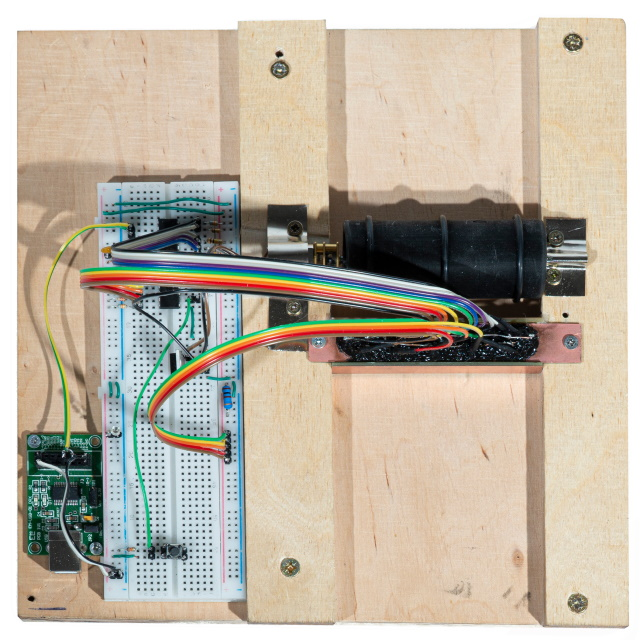
\includegraphics[width=0.75\linewidth]{img/topview}
			\caption{The device as seen from above.}
			\label{fig:topview}
		\end{center}
	\end{figure}
	
	Figure~\ref{fig:topview} shows the top view of the device. Linear motion is
	achieved by pulling the tape through an 80-millimeter-wide trough, which
	ensures that the tracks do not become misaligned with the read head. A DC
	motor coupled with a rubber-coated roller pulls the tape as it passes under
	the head.
	
	\newpage
	
	Suspended above the tape is the read head itself. It consists of 10
	phototransistors aligned with each of the tracks, as well as 5
	light-emitting diodes to provide controllable light conditions. The
	transistors are protected from overexposure by a layer of silicone coating
	from above and a heat shrink tube wrapped around the lens.
	
	\begin{figure}[h]
		\begin{center}
			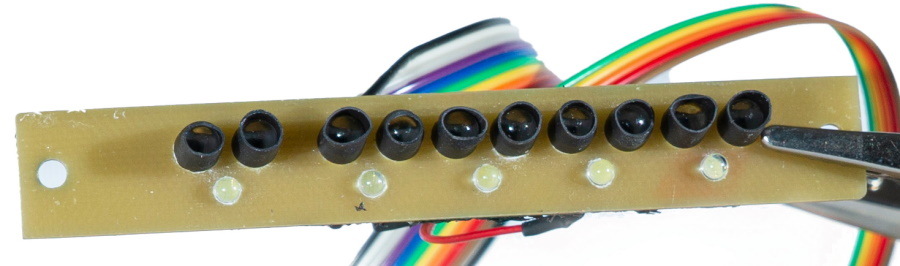
\includegraphics[width=0.75\linewidth]{img/readhead}
			\caption{The front face of the read head.}
			\label{fig:readhead}
		\end{center}
	\end{figure}
	
	To further protect the sensors from interference from outside light
	sources, the read head is enclosed within a dark chamber. The tape enters
	the chamber through a slit where the walls meet the trough. The slit also
	keeps the paper flush with the bottom of the trough.
	
	USB communication, being outside the scope of the project itself, is
	outsourced to an FT232 chip which emulates ordinary RS-232 communication
	over the Universal Serial Bus. The device appears as a serial port
	connection to the host computer. Because the FT232 chip does not come in a
	dual in-line package, a separate PCB is mounted alongside the breadboard.
	
	Being a peripheral device meant to be paired with a desktop computer, the
	reader has no external power source other than the USB port. The FT232 chip
	is configured to permit a maximum current of 500 mA, which is sufficient to
	power the motor even when it is stalled. The current consumed by the LEDs
	is very low (around 20 mA).
	
	The remaining two user-facing features of the device are the emergency stop
	button and the power LED. The button may be pressed to immediately halt a
	read session. The power LED is placed between the power rail and the ground
	rail to indicate that the device is powered on.
	
\end{document}
